                %!TEX program = xelatex
\documentclass[9pt, compress]{beamer}
\usetheme[sectionpage=progressbar]{metropolis}

\usepackage{subfigure} 
\usepackage{booktabs}  
\usepackage[scale=2]{ccicons}
\usepackage[T1]{fontenc}
\usepackage[utf8]{inputenc}
\usepackage{lmodern}
\usepackage{amsthm}
\usepackage{diagbox} %tabelas com barras
\usepackage{booktabs}
\usepackage{graphicx}			% Inclusão de gráficos
\usepackage[portuguese]{babel}
\usepackage{svg}
\newtheorem{teorema}{Teorema}


\graphicspath{{../figuras/}}

\author{\textbf{Matheus S. D'Andrea Alves}, \textbf{Uéverton dos Santos Souza} } 
\title{Coloração de Grafos$(r,\ell)$}
\subtitle{Coloração de Grafos$(r,\ell)$}
%\logo{}
\institute{\textbf{Universidade Federal Fluminense}}
\date{Julho 2018}
%\subject{}
%\setbeamercovered{transparent}
%\setbeamertemplate{navigation symbols}{}
\begin{document}
    \maketitle
    \begin{frame}{Agenda}
    \centering
        \tableofcontents
    \end{frame}
    \section{O problema}
    \begin{frame}{Conceitos iniciais}
      \begin{columns}
        \begin{column}{0.5\textwidth}
          \textbf{Grafo$(r,\ell)$}
          
          Um grafo que pode ser particionado em $r$ conjuntos independentes e $\ell$ cliques.
        \end{column}
        \begin{column}{0.5\textwidth}
          \textbf{Coloração dos vértices de um grafo}
          
          Uma coloração de um grafo $G$ é uma associação de uma cor entre $k$ cores a cada vértice do grafo de forma que, dado dois vértices vizinhos em $G$ eles não compartilhem uma cor, e $k$ seja o menor número de cores possíveis a respeitar tal restrição. 
        \end{column}
      \end{columns}
    \end{frame}
    \begin{frame}[standout]
      A PERGUNTA:
      
      Quando tal problema se torna NP-Completo? 
      
      Porque?
    \end{frame}
    \section{Nossa abordagem}
    \begin{frame}{A idéia}
      Construir uma dicotomia sobre a complexidade do problema, baseando-se nos valores de $r$ e $\ell$.
      
      Analisar os resultados e investigar padrões na dificuldade do problema.
    \end{frame}
    \begin{frame}{Primeiros passos}
      Começaremos dos seguintes fatos:
      \begin{itemize}
        \item Um grafo nulo (i.e. um Grafo$(0,0)$) é 0-colorível.
        \item 
        \item 
        \item 
         \item                                                                                                                
      \end{itemize}
    \end{frame}
    \begin{frame}{Primeiros passos}
      Começaremos dos seguintes fatos:
      \begin{itemize}
        \item Um grafo nulo (i.e. um Grafo$(0,0)$) é 0-colorível.
        \item Um grafo sem arestas (i.e. um Grafo$(1,0)$) é 1-colorível.
        \item 
        \item 
         \item                                                                                                                
      \end{itemize}
    \end{frame}
    \begin{frame}{Primeiros passos}
      Começaremos dos seguintes fatos:
      \begin{itemize}
        \item Um grafo nulo (i.e. um Grafo$(0,0)$) é 0-colorível.
        \item Um grafo sem arestas (i.e. um Grafo$(1,0)$) é 1-colorível.
        \item Um grafo bipartido (i.e. um Grafo$(2,0)$) é 2-colorível.
        \item 
         \item                                                                                                                
      \end{itemize}
    \end{frame}
    \begin{frame}{Primeiros passos}
      Começaremos dos seguintes fatos:
      \begin{itemize}
        \item Um grafo nulo (i.e. um Grafo$(0,0)$) é 0-colorível.
        \item Um grafo sem arestas (i.e. um Grafo$(1,0)$) é 1-colorível.
        \item Um grafo bipartido (i.e. um Grafo$(2,0)$) é 2-colorível.
        \item Um grafo completo (i.e. um Grafo$(0,1)$) é $k-colorivel$ onde $k$ é a quantidade de vértices de G.
        \item                                                                                                               
      \end{itemize}
    \end{frame}
    \begin{frame}{Primeiros passos}
      Começaremos dos seguintes fatos:
      \begin{itemize}
        \item Um grafo nulo (i.e. um Grafo$(0,0)$) é 0-colorível.
        \item Um grafo sem arestas (i.e. um Grafo$(1,0)$) é 1-colorível.
        \item Um grafo bipartido (i.e. um Grafo$(2,0)$) é 2-colorível.
        \item Um grafo completo (i.e. um Grafo$(0,1)$) é $k-colorivel$ onde $k$ é a quantidade de vértices do grafo.
        \item Um grafo split (i.e. um Grafo$(1,1)$) é $k-colorivel$ onde $k$ é a quantidade de vértices na clique máxima do grafo.
      \end{itemize}
    \end{frame}
    \begin{frame}{A mais}
      \begin{teorema}
        Coloração de Grafos(0,2) é Polinomial.
     \end{teorema}
     \begin{proof}
      Um grafo co-bipartido, é um grafo separável em 2 cliques em que todo vértice faz parte de alguma das cliques. A partir da literatura sabemos que um grafo co-bipartido é perfeito, isso é, seu número cromático é igual ao de sua clique máxima. 
      Já foi mostrado que encontrar a clique máxima em um co-bipartido é equivalente a se encontrar uma cobertura de vértices em seu complemento e portanto polinomial, ao encontrarmos a clique máxima sabemos que precisamos de seu número de vértices em cores para colorir tal grafo.
     \end{proof}
    \end{frame}
    \begin{frame}{A mais}
      \begin{teorema}
        Coloração de Grafos$(3,0)$ é Polinomial.
     \end{teorema}
     \begin{proof}
      Como sabemos que tal grafo é um Grafo(3,0) sabemos que o mesmo pode ser colorido com três cores.
      Saber se o mesmo pode ser colorido com duas ou uma cor é polinomial, portanto podemos afirmar que coloração em Grafos(3,0) é polinomial.
     \end{proof}
    \end{frame}
    \begin{frame}{A mais}
      \begin{teorema}
        Coloração de Grafos$(4,0)$ é NP-Completo.
     \end{teorema}
     \begin{proof}
      Sabemos que tal grafo é um Grafo(4,0), logo é possível o colorir com 4 cores.
      Precisamos descobrir se o mesmo pode ser colorido com menos cores; 
      Note que 3-coloração de planar é NP-Completo, e que existem subconjuntos de Grafos$(4,0)$ que são planares, logo coloração de Grafos$(4,0)$ é NP-Completo.
     \end{proof}
    \end{frame}
    \section{Primeiros resultados}
    \begin{frame}{Dicotomia parcial}
        \begin{table}[htb!]
          \center
          \begin{tabular}{l|*{7}c}
            \toprule
            \backslashbox{$r$}{$l$} & 0 & 1 & 2 & 3 & 4 & \ldots & n\\
            \midrule
            0 & \textit{P} & \textit{P} & \textit{P} & ? & ? & \ldots & ?\\
            1 & \textit{P} & \textit{P} & ? & ? & ? & \ldots & ?\\
            2 & \textit{P} & ? & ? & ? & ? & \ldots & ?\\
            3 & \textit{P} & ? & ? & ? & ? & \ldots & ?\\
            4 & \textit{NPc} & \textit{NPc} & \textit{NPc} & \textit{NPc} & \textit{NPc} & \ldots & \textit{NPc}\\
            $\vdots$ & $\vdots$ & $\vdots$ & $\vdots$ & $\vdots$ & $\vdots$ & $\ddots$ & \textit{NPc}\\
            n & \textit{NPc} & \textit{NPc} & \textit{NPc} & \textit{NPc} & \textit{NPc} & \ldots & \textit{NPc}\\
            \bottomrule
          \end{tabular}%
          \caption{Dicotomia parcial para coloração de Grafos$(r,\ell)$}
          \label{tab:tabela_part2dictrl}%
        \end{table}%
    \end{frame}
    \begin{frame}[standout]
      Como prosseguir?
    \end{frame}
    \section{A relação entre coloração e lista-coloração em Grafos$(r,\ell)$}
    \begin{frame}{A relação entre coloração e lista-coloração em Grafos$(r,\ell)$}
        \begin{teorema}
          Coloração é NP-Completo para Grafos$(r,\ell+1)$ quando lista coloração é NP-Completo para Grafo$(r,\ell)$
        \end{teorema}
    \end{frame}
    \begin{frame}{A relação entre coloração e lista-coloração em Grafos$(r,\ell)$}
        \textbf{Demonstração.}
        
        A prova consiste em mostrar que a solução do problema de lista coloração em um Grafo$(r,\ell)$ $G$, implica em uma solução para o problema de coloração em Grafos$(r,\ell+1)$ $H_G$.
        
        Para tanto, mostraremos que:
          \begin{itemize}
        \item Se um grafo G$(r,\ell)$ possui uma lista coloração própria então $H_G$ é k-colorível para k do tamanho da paleta $C$ (1).
		\item Se $H_G$ é k-colorível então G possui uma lista coloração própria (2).
      \end{itemize}
    \end{frame}
    \begin{frame}{A relação entre coloração e lista-coloração em Grafos$(r,\ell)$}
      \textbf{(1):}
      
      Seja $G$ um Grafo$(r,\ell)$ tal que cada vértice $v \in V(G)$ tenha uma lista de cores; 
      Cada lista tem pelo menos uma cor do seguinte conjunto: $C = \{c_1,c_2,c_3,...,c_k \}$. 
      \begin{center}
        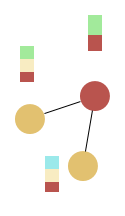
\includegraphics[scale=0.4]{presentation-G.png}
      \end{center}
    \end{frame}
    \begin{frame}
      Seja $G$ uma instância \textbf{sim} para o problema de lista coloração, construirémos uma clique $K$, onde cada vértice $u \in V(K)$ representa uma cor de $C$.
      \begin{center}
        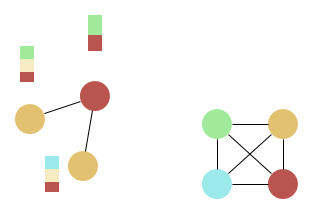
\includegraphics[scale=0.4]{presentation-K.png}
      \end{center}
      Note tque a clique $K$ tem exatamente $k$ vértices, portanto, podemos colorir $K$ com apenas $k$ cores, sem perda de generalidade assumiremos que $u_i \in K$ será colorido com a cor $c_i$.
    \end{frame}
    \begin{frame}  
      Suponha $H_G$ $= G \cup K$, e para cada vértice $u_i \in V(K)$ e todo vértice $v_j \in V(G)$ adicione uma aresta $(u_i,v_j) $ em $H_G$ se e somente se $c_i$ não é uma cor pertencente a lista de $v_j$.
      \begin{center}
        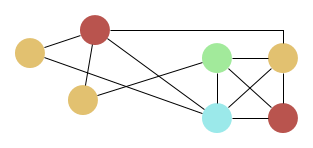
\includegraphics[scale=0.4]{presentation-H.png}
      \end{center}   
      Usando tal coloração, a coloração de $K$ não conflita para a coloração encontrada para $G$, temos assim uma coloração para $H_G$. 
    \end{frame}
    \begin{frame}{A relação entre coloração e lista-coloração em Grafos$(r,\ell)$}
      \textbf{(2):}
      
      Sabemos que o grafo $H_G$ é um grafo$(r,\ell+1)$ e possui uma k-coloração. Onde $K$ é a clique máxima de $H_G$.
      Seja $k$ o número de vértices em $K$.
      
      Perceba que a remoção de $K$ de $H_G$ (que se tronará $G$) não afeta sua coloração, perceba que para os restantes vértices $v \in V(G)$ construímos suas listas baseando-se em seus não vizinhos em $K$ portanto a coloração adquirida em $H_G$ ainda é válida em $G$ por construção.
      
      Dessa forma mostramos que, se $H_G$ é k-colorível, $G$ é lista-colorível.
      $\qed$
    \end{frame}
    \begin{frame}{Corolários}
      Com o resultado obtido podemos afirmar que:
      \begin{itemize}
        \item Coloração em Grafos$(1,2)$ é NP-Completo.\newline Deriva da demonstração de NP-Completude para lista coloração em Split mostrado por Jensen et al. em \textit{"Generalized coloring for tree-like graphs"}.
        \item Coloração em Grafos$(2,1)$ é NP-Completo.\newline Deriva da demonstração de NP-Completude para lista coloração em bipartidos mostrado por Fellows et al. em \textit{"List Coloring and Precoloring Extension are W[1]-hard parameterized by treewidth"}.
        \item Coloração de Grafos$(0,3)$ é NP-Completo.
        \newline Deriva da demonstração de NP-Completude para lista coloração em Grafos$(0,2)$ demonstrado por Jensen et al. em \textit{"Complexity results for the optimum cost chromatic partition problem"}.
      \end{itemize}
    \end{frame}
    \begin{frame}{ Peculiaridade do Grafo$(2,1)$ }
      É trivial notar que essa classe de grafo possui um limite superior e um inferior para sua coloração ($K+1$ e $K$ respectivamente), porém apesar das restrições é NP-Completo determinar qual delas é a correta.
    \end{frame}
    \section{Resultados clássicos}
    \begin{frame}{Complexidade computacional de Coloração em Grafoa$(r,\ell)$}
        Os resultados encontrado preenchem a dicotomia.
        
        \begin{table}[htb!]
          \center
          \begin{tabular}{l|*{7}c}
            \toprule
            \backslashbox{$r$}{$l$} & 0 & 1 & 2 & 3 & 4 & \ldots & n\\
            \midrule
            0 & \textit{P} & \textit{P} & \textit{P} & \textit{NPc} & \textit{NPc} & \ldots & \textit{NPc}\\
            1 & \textit{P} & \textit{P} & \textit{NPc} & \textit{NPc} & \textit{NPc} & \ldots & \textit{NPc}\\
            2 & \textit{P} & \textit{NPc} & \textit{NPc} & \textit{NPc} & \textit{NPc} & \ldots & \textit{NPc}\\
            3 & \textit{P} & \textit{NPc} & \textit{NPc} & \textit{NPc} & \textit{NPc} & \ldots & \textit{NPc}\\
            4 & \textit{NPc} & \textit{NPc} & \textit{NPc} & \textit{NPc} & \textit{NPc} & \ldots & \textit{NPc}\\
            $\vdots$ & $\vdots$ & $\vdots$ & $\vdots$ & $\vdots$ & $\vdots$ & $\ddots$ & \textit{NPc}\\
            n & \textit{NPc} & \textit{NPc} & \textit{NPc} & \textit{NPc} & \textit{NPc} & \ldots & \textit{NPc}\\
            \bottomrule
          \end{tabular}%
          \caption{Dicotomia de complexidade para coloração em Grafos$(r,\ell)$}
          \label{tab:tabela_dictrl}%
        \end{table}%
    \end{frame}
    \begin{frame}[standout]
      Como parametrizar a coloração de Grafos$(r,\ell)$?
    \end{frame}
    \section{Parametrizado pelo tamanho das partições}
    \begin{frame}{A idéia}
          Usar o tamanho das partições de um Grafo$(2,1)$ como parâmetros do problema.
    \end{frame}
    \begin{frame}{Parametrização}
      \large{Parametrização de Grafo$(2,1)$ pelo tamanho do menor independente}
      \normalsize\newline\newline
            
      Sabemos que podemos transformar esse problema em lista coloração de bipartido.
      
      Fellows mostrou que lista-coloração é w[1]-difícil para bipartidos quando parametrizado pelo tamanho do menor independente.
      
      Portanto coloração é w[1]-difícil quando parametrizado pelo tamanho do menor independente em um Grafo$(2,1)$.
    \end{frame}
    \begin{frame}{Parametrização}
    \large{Parametrização de Grafo$(2,1)$ pelo tamanho do maior independente.}
      \normalsize\newline\newline
            
      Sabemos que podemos transformar esse problema em lista coloração de bipartido.
      
      Em uma lista coloração de bipartido, se um vértice possui uma lista com mais cores do que o tamanho de sua vizinhança, ele sempre terá disponível uma cor para sua coloração, podemos portanto remover esse vértice do grafo sem alterar sua coloração.
      
      Observe que isso implica que após a remoção de todos os vértices com esse padrão o tamanho das listas está agora limitado por uma função de $k$, portanto aplicar um algoritmo de força bruta nos dá um algoritmo FPT.
     \end{frame}
     
    \section{Parametrização pelo tamanho da clique}
     \begin{frame}{Pre-coloring extension}
      \large{Pre-coloring extension}
      \normalsize\newline\newline
      
	      \textbf{Entrada:}  Um grafo G onde alguns vértices já possuem uma coloração definida com cores escolhidas dentre k possíveis cores.
	      
	      \textbf{Pergunta:}  É possível estender a coloração já existente para todo o grafo sem que dois vértices adjacentes possuam a mesma cor?
     \end{frame}
     
     \begin{frame}{3-lista coloração em grafos bipartidos é NP-Completo.}
    \large{3-lista coloração em grafos bipartidos é NP-Completo.}
      \normalsize\newline\newline
            
      Tendo um grafo $G$ e uma paleta $C$ pertencente a uma instância $P$ de \emph{Pre coloring extension}.
      
      Formamos um grafo $G'$ usando todo vértice pré-colorido $v \in V(G)$ atribuindo ao mesmo uma lista com sua cor de $G$ em $G'$, aos demais vértices de $G$ criamos um vértice com lista contendo todos as cores de $C$ e mantendo sua vizinhança.
      
      Uma coloração possível para $G$ implica em uma coloração possível para $G'$ , já que nos basta atribuir aos vértices em $G'$ as mesmas cores atribuídas em $G$. De forma análoga, uma lista coloração possível em $G'$ implica em uma coloração possível em $G$.
      
      
     \end{frame}
     \begin{frame}{Parametrização.}
    \large{Parametrização pelo tamanho da clique.}
      \normalsize\newline\newline
            
      Para demonstração da intratabilidade parametrizada, basta retornarmos à transformação do problema de coloração em Grafo$(2,1)$ em lista coloração de bipartido.
      
      Estamos tentando parametrizar a resolução de lista coloração de bipartido pelo tamanho da paleta de cores, que mostramos ser inviável anteriormente.
      
      Portanto esse problema é para-NP-Completo quando parametrizado pelo tamanho da clique.
      
     \end{frame}
     \section{Parametrização pela vizinhança da clique}
     \begin{frame}{Observações}
       Usando um Grafo$(2,1)$ onde a partição da clique também é a clique máxima e tem tamanho 3, nosso problema se torna o problema de 3-lista-coloração em bipartido.
       
       3-coloração de bipartido é Polinomial.
       
       2-coloração de bipartido é Polinomial 
       
       3-lista-coloração de bipartido é NP-Completo.
       
       O que ocorre quando o número de vértices com listas de tamanho 1, 2 e 3 variam? 
     \end{frame}
     \begin{frame}{Sobre a vizinhança da clique}
       Observe que, se um nó não é vizinho de nenhum vértice na clique, após a redução esse vértice tem lista de tamanho três. Todo vértice vizinho a clique, após a transformação tem vértice com lista de tamanho $3-n$ onde $n$ é o número de seus vizinhos na clique.
       
       Um vértice nunca terá uma lista de tamanho 0.
     \end{frame}
     \begin{frame}{Vértices com listas de tamanho um}
       \begin{teorema}
       Seis vértices com lista de tamanho um são suficientes para que lista coloração em bipartido seja NP-completo.
       \end{teorema}
       \textbf{Demonstração.}
       
       Sabemos que em nosso problema temos dois conjuntos independentes, $r_1$ e $r_2$, também é verdade que exceto pelos citados seis vértices todos os outros tem listas de tamanho três, os vértices de $r_1$ podem estar ligados arbitrariamente aos de $r_2$. Observe a disposição de tais vértices na figura a seguir, chamaremos tal esquema de $\mathcal{N}$.
     \end{frame}
     \begin{frame}
        
        \begin{figure}[H]
		        \centering
		        \fontsize{4}{10}
		        \includesvg[scale=0.4]{seis-vertices-lista-um.svg}
		        \caption{Esquema de vizinhança formado por 6 vértices com distintas listas tamanho 1. }
		        \label{fig:seis-vertices-lista-um}
        \end{figure}
    
        Agora, através do gadget da figura seguinte mostraremos como a presença de vértices com distintas listas de tamanho um influencia na coloração de sua vizinhança comum.
      \end{frame}
    \begin{frame}
   \begin{figure}[H]
      \begin{subfigure}
        \centering
		    \includesvg[scale=0.4]{gadget-1.svg}
      \end{subfigure}
      \begin{subfigure}
        \centering
		    \includesvg[scale=0.4]{gadget-2.svg}
      \end{subfigure}
      \begin{subfigure}
        \centering
		    \includesvg[scale=0.4]{gadget-3.svg}
      \end{subfigure}
      \caption{Gadget com vértices de lista um reproduzindo vértice de lista um em vértice de lista três}
      \label{fig:gadget}
  \end{figure}

      Com o gadget apresentado é possível conduzir à escolha de uma cor para um vértice com lista tamanho três dado que a única coloração possível para o gadget é a coloração aonde a cor desejada ocorre.
    \end{frame}
    \begin{frame}
      Utilizando esse gadget é possível transformar uma instância de PreColoring Extension em bipartidos em uma de lista coloração em bipartido, basta para tanto pegarmos os vértices do Grafo $G$ que estão pré-coloridos e criar um vértice equivalente em um grafo $G'$ com listas tamanho três, os ligando aos vértices de $\mathcal{N}$ e mantendo a bipartição de forma a excitar a cor que este vértice possuia em $G$, os demais vértices são mapeados para vértices com listas tamanho três, mantendo sua vizinhança equivalente a em $G$.

      Assim se a lista coloração for possível em $G'$ basta escolher as mesmas cores para colorir $G$, o mesmo se aplica a contraparte da demonstração. Dessa forma mostramos que com seis vértices com distintas listas tamanho um, encontrar uma lista coloração para tal grafo é NP-Completo. $\qed$
    \end{frame}
     \begin{frame}{Encontrando a quantidade mínima}
       \begin{teorema}
       Lista coloração em bipartido é de solução trivial quando há apenas um vértice de lista tamanho um.
       \end{teorema}
       \begin{proof}
       Sabemos que além do vértice citado todos os outros vértices têm listas de tamanho três dessa forma basta que o conjunto independente no qual tal vértice está inserido seja colorido com a única cor escolhida para o vértice e o conjunto independente sobrante pode ser colorido com qualquer cor.
       \end{proof}
       \end{frame}
       \begin{frame}
       \begin{teorema}
       Lista coloração em bipartido é de solução linear quando existem dois vértices de lista tamanho um.
       \end{teorema}
       \begin{proof}
        Para essa demonstração é necessária a observação em que existem duas possíveis configurações para essa instância:
        \begin{itemize}
          \item Ambos os vértices pertencem ao mesmo conjunto independente.
          \item Os vértices pertencem a conjuntos distintos.
        \end{itemize} 
        No primeiro caso pode-se adaptar a estratégia de coloração anterior para a solução. Para tanto basta colorir tais vértices com suas cores disponíveis e o conjunto independente ao qual pertencem com a cor de algum deles, e o conjunto sobressalente com a cor restante.
 
        No segundo caso, a coloração também é simples. Se tais vértices tem cores distintas basta colorir seus respectivos conjuntos com a mesma cor. Se não, como temos três cores podemos colorir os vértices com a cor 1, um conjunto com a cor 2 e os demais vértices com a cor 3.
       \end{proof}
     \end{frame}
     \begin{frame}
       \begin{teorema}
         Três vértices com lista de tamanho um são suficientes e necessários para que lista coloração em bipartido seja NP-completo.
       \end{teorema}
       \begin{proof}
        Usando o gadget apresentado anteriormente, dois vértices $v$ com lista um em um vértice $u$ com lista três são capazes de reproduzir um vértice de lista um através da retirada da lista de $u$ as únicas possíveis cores para $v$, sendo assim tendo três vértices de distintas listas tamanho um, é possível obter seis vértices de lista um (com três listas distintas de cada lado) e reproduzir a redução mostrada no caso com seis vértices, que nos mostra a NP-Completude desse problema.
       \end{proof}
     \end{frame}
     \begin{frame}{Vértices com listas de tamanho dois}
       Como já visto o problema é de trivial solução quando todos os vértices tem listas de tamanho três, portanto precisamos ainda encontrar qual número de vértices de tamanho dois onde o problema se mantém NP-Completo.
       \begin{teorema}
         Seis vértices com listas tamanho 2 são necessários e suficientes para que lista-coloração em bipartido seja NP-Completo.
       \end{teorema}
       \textbf{Demonstração.}
       
 
       Se um conjunto independente contém apenas dois vértices com listas tamanho dois, todos os vértices nesse conjunto compartilham uma cor em suas listas, podendo colorir tal conjunto com essa cor.
       
        Todos os outros vértices ainda têm pelo menos uma cor disponível para sua coloração podendo ser colorido com ela. 
       
       Para completar nossa demonstração basta portanto, encontrar uma configuração onde o problema de lista coloração permanece NP-Completo.
 
       Para tanto nos é interessante agora a vizinhança entre os vértices com lista dois, iremos isolar as instâncias em alguns casos.  
       
     \end{frame}
     \begin{frame}{Vizinhança de algum vértice é tamanho um}
        Nesse caso podemos notar que independentemente do vértice $v \in r_1$ e seu vizinho $u \in r_2$, eles sempre compartilharão uma cor, colorimos o vértice $u$ com tal cor, além disso como conhecemos a vizinhança de $v$ sabemos que nenhum outro vértice é vizinho deste, podemos então colorir os restantes vértices de $r_2$ com a cor de $v$, dessa forma uma das três cores ainda resta e podemos a usar para colorir o restante do $r_1$, independente das ligações entre os demais vértices de $r_1$ e $r_2$.
     \end{frame}
     \begin{frame}
       \begin{figure}[H]
         \centering
         \fontsize{4}{10}
         \includesvg[scale=0.4]{1-edge.svg}
         \caption{Demonstração de coloração para vizinhança de tamanho um.}
       \end{figure}
     \end{frame}
     \begin{frame}{Um vértice têm vizinhança tamanho dois, e compartilha uma cor com ambos os vizinhos}
       Aqui podemos executar o seguinte algoritmo, sem perda de generalidade pinte os vértices vizinhos à $v \in r1$ com a cor compartilhada, novamente por conhecermos a vizinhança do vértice $v$ podemos pintar ele e os demais vértices de $r_2$ com a cor restante, dessa forma ainda nos resta uma cor para colorir os demais vértices de $r_1$.
     \end{frame}
     \begin{frame}
       \begin{figure}[H]
     \centering
     \fontsize{5}{10}
     \includesvg[scale=0.4]{2-edge.svg}
     \caption{Demonstração de coloração para vizinhança de tamanho dois com cores compartilhadas.}
   \end{figure}
     \end{frame}
     \begin{frame}{Todo vértice tem vizinhança de tamanho dois e nenhuma vizinhança possui uma cor em comum}
       As restrições impostas a esse caso nos levam a uma única possível estrutura $\Gamma$ onde suas duas possíveis colorações são intercambiáveis.
       
       Portanto se mostra verdade que podemos excitar uma cor qualquer em outro vértice de lista tamanho três se o ligarmos a dois dos três vértices presentes no independente oposto sem ferir a bipartição do grafo.
     \end{frame}
     \section{Conclusão}
     \begin{frame}[standout]
       OBRIGADO!
       
       Perguntas?
     \end{frame}
\end{document}
